\chapter{Experiments} 
\label{chapter:experiments} 

This chapter mainly focuses on answering the following questions:
\begin{itemize}
\item What are possible ways of using distantly supervised data?
\item Can Distant Supervision improve upon the results of supervised training?
\item Can a neural network architecture that is developed in a general domain setting be used to tackle the medical domain - a domain which is usually handled with lots of Natural Language Processing features?
\item Which embedding types are best-suited for relation extraction in different domains?
\end{itemize}

The chapter is divided into two parts - one is dedicated to the supervised learning on manually labeled 
datasets and serves to demonstrate the baseline, while the second one contains experiments with Distant Supervision. Each of them is divided into a part for the general domain and a part for the medical domain. Overall two supervised 
datasets for each of the domains were evaluated and one dataset per domain is created for evaluating Distant Supervision. The scheme of all the experiments can be seen in the Figure \ref{fig:exp-schema}.

\begin{figure}
\centering
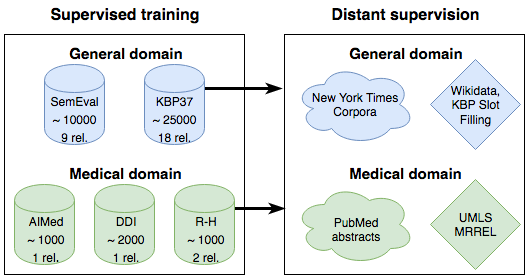
\includegraphics[width=\textwidth]{chapter4_experiments/images/exp-schema.png}
\caption[Experiments scheme]{Scheme of conducted experiments for the network evaluation.}
\label{fig:exp-schema}
\end{figure}

In order to find the best network configuration, one 4-fold validation experiment was performed once for each domain. The parameters that were 
tuned were the length of the embeddings, both for words and for distances, and the type of the 
word embedding. The grid consisted of \{30, 40, 50, 70\} for distance embeddings length, \{300, 400\} for word embeddings length and \{Swivel, GloVe, Word2Vec\} for embedding types. In order to make the model universal, parameters for all the other experiments were fixed to the found via cross-validation.

\section{Supervised training evaluation, general domain}
The goal of experiments in this section is to validate the implementation of the network by 
comparing with the results achieved in \cite{DBLP:journals/corr/SantosXZ15} and prove the quality 
of the network by applying it to the other supervised dataset in general domain. 
The experiments in general domain use text corpora and relations from unspecific sources, such as 
Wikipedia, Freebase and news corpora. The biggest problem in the general domain setting is ambiguity. Named entities can have multiple meanings in different contexts and two entities can also belong to multiple relation types. Generally speaking, detecting one of the general domain relations is a 
challenging task even for humans. For example, given the entity pair ''The Lord of The Ring'' and 
''The Return of the King'' it is hard to decide whether the relation between them is 
''Member-Collection'' or ''Component-Whole''.
\subsection{SemEval 2010, Task 8}
The ''SemEval 2010, Task 8'' (SemEval) dataset is one of the most common datasets for Relation Extraction evaluation. As the name implies, it was part of the SemEval 2010 competition \cite{hendrickx2009semeval}, namely for Task 8, and it was also the dataset that \cite{DBLP:journals/corr/SantosXZ15} used for evaluating and training their model. Since the models in this thesis built upon the model from \cite{DBLP:journals/corr/SantosXZ15}, the SemEval dataset was used to verify the model implementation.

The dataset contains approximately 10000 labeled sentences. The labels are nine relation types and 
the ''Other'' class that includes different relations not included in the main ones. The examples were 
manually collected from the web and annotated in three rounds, so all the annotators would agree 
on the label given to the sentence. The classes of the relations are following (description is taken 
from \cite{hendrickx2009semeval}):

\textit{\begin{enumerate}
  \item \textbf{Cause-Effect } An event or object leads to an effect. Example: those 
  $<e2>$cancers$</e2>$ were 
  caused by radiation $<e1>$exposures$</e1>$.
  \item \textbf{Instrument-Agency} An  agent  uses  an  instrument. Example: $<e1>$phone$</e1>$ $<e2>$operator$</e2>$.
  \item \textbf{Product-Producer} A producer causes a product to exist. Example: a $<e2>$factory$</e2>$ manufactures $<e1>$suits$</e1>$.
  \item \textbf{Content-Container} An object is physically stored in a delineated area of space. 
  Example: a $<e2>$bottle$</e2>$ full of $<e1>$honey$</e1>$ was weighed.
  \item \textbf{Entity-Origin} An entity is coming or is derived from an origin (e.g., position or 
  material). Example: $<e1>$letters$</e1>$ from foreign $<e2>$countries$</e2>$.
  \item \textbf{Entity-Destination} An entity is moving towards a destination. Example: the $<e1>$boy$</e1>$ 
  went to $<e2>$bed$</e2>$.
  \item \textbf{Component-Whole} An object  is a  component  of a  larger whole. Example: my 
  $<e2>$apartment$</e2>$ has a large $<e1>$kitchen$</e1>$.
  \item \textbf{Member-Collection} A member forms a nonfunctional part of a collection. 
  Example: there are many $<e1>$trees$</e1>$ in the$<e2>$forest$</e2>$.
  \item \textbf{Message-Topic} A message, written or spoken, is about a topic.  Example: the 
  $<e1>$lecture$</e1>$ was about $<e2>$semantics$</e2>$.
\end{enumerate}}

It should be noted, that since sentences in the dataset can contain entities in the different order, 
there are finally nineteen classes of relations - two for each of the nine main and ''Other''.
Some of the relations are closely connected in order to test the ability to make fine-grained 
distinctions, e.g. Content-Container, Component-Whole, Member-Collection.

For evaluation of the result achieved by a solver, there is a specially written evaluator, that calculates 
different characteristics of the predictions made.  According to the description in the code of the scorer:
\begin{displayquote}
     \textit{The scorer calculates and outputs the following statistics:
       \begin{enumerate}
         \item confusion matrix, which shows
          \begin{itemize}
            \item the sums for each row/column: -SUM-
            \item the number of skipped examples: skip
            \item the number of examples with correct relation, but wrong directionality: xDIRx
            \item the number of examples in the answer key file: ACTUAL ( = -SUM- + skip + xDIRx )
          \end{itemize}
          \item accuracy and coverage
          \item precision (P), recall (R), and F1-score for each relation
          \item micro-averaged P, R, F1, where the calculations ignore the Other category
          \item macro-averaged P, R, F1, where the calculations ignore the Other category
       \end{enumerate}}
       
     \textit{Note that in scores (4) and (5), skipped examples are equivalent to those classified as Other.
     So are examples classified as relations that do not exist in the key file (which is probably not optimal).}

     \textit{The scoring is done three times:
     \begin{enumerate}
       \item as a (2*9+1)-way classification
       \item as a (9+1)-way classification, with directionality ignored
       \item as a (9+1)-way classification, with directionality taken into account
     \end{enumerate}}
          
     \textit{The official score is the macro-averaged F1-score for (3).}
\end{displayquote}(taken from the commentaries in the scorer code)

\subsection{KBP37}
The KBP37 dataset \footnote{\url{https://github.com/zhangdongxu/kbp37}}, as it was called in the paper \cite{DBLP:journals/corr/ZhangW15a}, was used 
to check up the results of solving the problem in the general domain with a fully supervised 
approach. In contrast to the original paper, the model was evaluated on the SemEval as well as on the KBP37 dataset, to test its perform on other types of relations and entities and to confirm the applicability of the network structure onto different datasets.

The KBP37 dataset is a revision of MIML-RE annotation dataset from \cite{angeli2014combining}, that 
was built from a subset of Wikipedia articles by manual annotation. It contains approximately 25000 labeled sentences. The  
 following changes were made by the authors of \cite{DBLP:journals/corr/ZhangW15a} to adapt it to the description of the SemEval task 8:
\begin{itemize}
  \item Added direction to the relations, i.e. 'per:employee-of(e1,e2)' and 'per:employee-of(e2,e1)' 
  instead of simply 'per:employee-of'. This is done for all the relations except for 'no-relation'
  \item Balance the dataset, to exclude the relations that have less than 100 examples for each of 
  the directions. Also, $80\%$ of 'no-relation' examples are discarded
  \item After that, examples are shuffled and split into three parts, $70\%$ for training, $10\%$ for 
  development and the rest for testing.  
\end{itemize}
After all the modifications, the dataset consists of 18 directional relations, that will result in 37 classes for 
recognition (two directions for each of 18 and 'no-relation'). This dataset is more complex than SemEval. It has longer sentences (almost twice longer than the 
longest in SemEval) and also it has multi-relational pairs that are of course common in 
the real world, but still hard to tackle. Also, it can be observed that both relations and entities in this dataset are more 
specific. So most of the entities are company or people names, compared to 
SemEval task, where entities were mostly general objects and people categories (e.g. boy, witch). 
Furthermore, the relations are very specific, e.g. there are three different classes for placement of 
headquarters of a company dependent on what it is - a city, a state or a country.

One more aspect of the dataset should be mentioned. Initially, it was labeled by crowdsourcing and the labels 
were given with different confidence level. But still, the authors of \cite{DBLP:journals/corr/ZhangW15a} took all of the sentences for the training 
and evaluation. Thus there could be found very imprecise examples, such as:

\textit{It was because of $<e1>$Abu Talib$</e1>$ 's ( a.s. ) good fortune that apart from $<e2>$his$</e2>$ ancestral services and prestige he also inherited from sons of Ismail ( a.s. ) high status and courage. \textbf{per:alternate-names(e2,e1)}}

During applying the network to KBP37 'no-relation' class was renamed to 'Other' for consistency 
with SemEval. The evaluation was performed by adapting the script from the SemEval 2010 Task 8.

\subsection{Results}
Cross-validation experiments were held on SemEval dataset. All parameters, that are not specified as changing for validation testing, were set to the values 
that are recommended in \cite{DBLP:journals/corr/SantosXZ15}. So, an embedding for class 
''Other'' was not trained, the number of filters was set to 1000, the size of the convolution window was set to 3, 
regularisation rate was 0.001 and learning rate was 0.25, decreasing by dividing by the number
of the epoch. Each experiment lasted 15 epochs. The F1-scores of validation experiments can be  
seen in the Table \ref{tab:val-semeval}. According to the experiment, the best configuration used for all the other experiments in the general domain is a combination of Word2Vec embeddings of the length 300 with distance embeddings of the length 30.

\begin{table}
        \centering
        \begin{tabular}{|c|c|c|c|c|c|c|}
          \hline
            & \multicolumn{3}{|c|}{Word embedding size 300} & \multicolumn{3}{|c|}{Word embedding size 400} \\\hline
            Dist. emb. & GloVe & Word2Vec & Swivel & GloVe & Word2Vec & Swivel  \\\hline
            \multicolumn{1}{|c|}{30} & 78.83 & \textbf{81.96} & 72.20 & 77.23 & 60.48 & \textit{80.17} \\\hline
            \multicolumn{1}{|c|}{40} & 78.45 & \textit{81.59} & 72.03 & 76.62 & 61.16 & \textit{80.16} \\\hline
            \multicolumn{1}{|c|}{50} & 77.98 & \textit{81.65} & 71.50 & 76.46 & 62.39 & \textit{80.39} \\\hline
            \multicolumn{1}{|c|}{70} & 77.68 & \textit{81.52} & 71.10 & 76.50 & 62.72 & \textit{79.95} \\\hline
        \end{tabular}
        \caption[Cross-validation for the general domain]{F1-scores of the cross-validation experiments on SemEval dataset obtained with the official scorer of the competition. Every score is an averaged score of four experiments. With \textit{italics} emphasised largest score for each setup and with \textbf{bold} largest in the whole validation.}
        \label{tab:val-semeval}
    \end{table}

All the train accuracies reached 99.99 - 100 percents, except for Word2Vec of length 400, that gave 96-98 percents. Interesting to note, that independently of the size for the distances embeddings Word2Vec is constantly better than any other embedding type for length 300, but with length 400 Swivel is a stable winner.  Also can be noticed, that Swivel embeddings show better results with higher dimensionality, while results with GloVe on the other hand drop. But it should be remembered, that a pre-trained version for GloVe of the length 300 was used. For validating the hypothesis that available pre-trained embeddings are of a higher quality than locally trained ones, the same experiment with locally trained embeddings was held. The results can be seen in the Table \ref{tab:local-val-semeval}. These results show slightly lower results for GloVe of the length 300, but much lower for Word2Vec.

\begin{table}
        \centering
        \begin{tabular}{|c|c|c|c|}
          \hline
            & \multicolumn{3}{|c|}{Word embedding size 300} \\\hline
            Dist. emb. & GloVe & Word2Vec  \\\hline
            \multicolumn{1}{|c|}{30} & 76.89 & 62.71 \\\hline
            \multicolumn{1}{|c|}{40} & 76.48 & 63.72 \\\hline
            \multicolumn{1}{|c|}{50} & 76.80 & 63.31 \\\hline
            \multicolumn{1}{|c|}{70} & 76.47 & 63.84 \\\hline
        \end{tabular}
        \caption[Cross-validation for the general domain on locally trained embeddings]{F1-scores of the cross-validation experiments on SemEval dataset performed with locally trained versions of word embeddings.}
        \label{tab:local-val-semeval}
    \end{table}

 The best configuration obtained in \cite{DBLP:journals/corr/SantosXZ15} was combination of Word2Vec of the length 400 with distance embeddings of the length 70. With this setup they got the best result of $F1=84.1$. But conducted cross-validation experiment showed that F1-scores for Word2Vec 
of the length 400 are worse than all other configurations. The training of these embeddings was done 
according to the scheme proposed in the paper \cite{DBLP:journals/corr/SantosXZ15}, but 
still, score for this configuration is not the highest. Even though training scores for 
these experiments might give an idea, that training can be continued in order to get better 
results, further training does not change the score anymore. The score just fluctuates around 
certain achieved values, going lower and falling back, but not going higher.

The best configuration according to the validation experiments was tested on the test set of 
SemEval2010 Task8 dataset and KBP37 test dataset. The score achieved is compared to other scores in the Table 
\ref{tab:test-superv-general}. It can be concluded, that model works approximately with same 
results as in the original paper, so the implementation is correct. Also, it was nice to notice that 
results achieved with Convolutional Neural Network are higher than with Recurrent Neural Network from 
\cite{DBLP:journals/corr/ZhangW15a}.

\begin{table}
  \begin{center}
 \begin{tabular}{ | c | c | c | }
    \hline
    Classifier & SemEval2010 & KBP37 \\ \hline
    CR-CNN \cite{DBLP:journals/corr/SantosXZ15} & 84.1 & - \\ \hline
    RNN \cite{DBLP:journals/corr/ZhangW15a} & 79.6 & 58.8 \\ \hline
    Supervised Ranking CNN & \textbf{84.39} & \textbf{61.26} \\ \hline
    \end{tabular}
\caption[General domain supervised experiments results]{F1-scores for testing datasets.}
\label{tab:test-superv-general}
\end{center}
\end{table}

Thus, the experiment proved the correctness of the implementation. Also, the result of the evaluation
 proves that the model does not perform well only on the one dataset 
it was constructed for, but also on other datasets as well.

\subsection{Interpretation}
In order to make the work of the network more transparent and explainable, several additional 
experiments were made.

\paragraph{Representative trigrams} 
\label{par:gen-superv-repr-trig}
As it is described in Subsection \ref{subs:repr-trigr} representative 
trigrams were extracted for every of 18 classes in SemEval2010 and 36 classes in KBP37. 

The five representative trigrams with the highest values for each of the classes of SemEval2010 
dataset can be seen in the Table \ref{tab:repr-trigr}. Should be noticed, that sometimes trigram 
can be in the beginning or in the end of a sentence or include some punctuation signs. In such 
cases trigram will not include exactly three words but two or even only one. Also, for one direction of 
''Entity-Destination'' relation there is only one trigram, because the training dataset contained only 
one example labeled with this class.

\begin{table}
  \begin{center}
 \begin{tabular}{ | p{2cm} | p{5cm} |  p{5cm} | }
    \hline
    Relation & (e1, e2) & (e2, e1) \\ \hline
     Message-Topic & the news that, contains a description, laws defining, of publications discussing & topic of conversation, topic of discussion, been reflected in, been discussed in \\ \hline
     Cause-Effect & common cause of, that resulted in, main causes of, leading causes of & are caused by, been caused by, was caused by, is caused by, damage caused by \\ \hline
     Component-Whole & part of the, the crank of, lid of the, handgrip of the, part of this & the knife blade, has a coil, my ear lobes, the mouse button \\ \hline
     Entity-Origin & was distilled from, is derived from, popped out of, is distilled from, away from the & the source of, of wheat liquor, some strawberry syrup, on rye liquor \\ \hline
     Member-Collection & essays collected in, in the army, the head of, of the team, a soldier joins & a confederacy of, a cooperative of, a federation of, a cabal of, covey of partridges \\ \hline
     Instrument-Agency & a crane operator, the elevator operator, are used by , a forklift operator & with a spoon, the author uses, a person applies, potter 's wheel \\ \hline
     Product-Producer & produced by the, book 's author, created by the, from the author, founded by a & the factory's, issued a statement, factory's output, the designer's \\ \hline
     Entity-Destination & poured flour into, was put into, were released into, poured water into, are migrating into & and steadily climbs \\ \hline
     Content-Container & in a box, in a suitcase, in a crate, in a bottle, money was in & a bottle full, a bottle with, a suitcase full, a suitcase with, envelope contained a \\ \hline
    \end{tabular}
\caption[Representative trigrams, SemEval dataset]{Representative trigrams according to the network for SemEval2010 Task8 dataset classes.}
\label{tab:repr-trigr}
\end{center}
\end{table}

Certain conclusions can be made from these lists of trigrams extracted for the relations. First, most of them make sense from the point of view of a human reader. So if a human will try to classify relation ''cause-effect'' most probably exactly phrases, like \textit{resulted in} or \textit{caused by}, would be a sign that a sentence contains this relation. Second, some of the trigrams still contain somehow specific words, for example, ''bottle'', ''suitcase'', ''box'' for ''content-container'' relation. In order to understand the origination of such words, the most frequent entities in the dataset were looked up. And it revealed, that ''suitcase'' for example is a very frequent entity for ''content-container'' examples, with 21 out of 433 examples for one direction and 31 out of 181 for the other. Thus, if some word appears very frequently in all examples for the relation it most probably will be among representative trigrams.

Most of the trigrams extracted for KBP37 dataset are not very general. For example, for class 
cities-of-residence the most valued 
trigrams are ''in Los Angeles, in Detroit Michigan, in London in, to London to'', so basically 
universal parts are only ''in'' and ''to'', everything else is very specific to the dataset. One can 
assume that this happens because of the very close meanings and entity pairs in all examples 
for one particular class. At the same time, for example, class ''founded-by'' is quite generalisable 
through its representative trigrams, such as ''founder of the, created google in, founder of gome, founders of dow''. Another explanation that entities in this dataset are mostly proper names, so 
in order to recognise relation it would be easier to learn the own names for example. Moreover, a 
look into the dataset reveals that sentences for one and the same relation really do not have a lot of 
''characteristic'' words in common, like it was in the case of SemEval dataset. It is also noticeable, that overall Precision is higher than Recall, i.e. network learned some specific details, 
that allow distinguishing some examples nicely, but not to see all possible examples of the 
relation.
\\\textbf{org:founded-by} \textit{founder huang guangyu, the congregation of, founder bill gates, international pictures co-founder, founder of the, schlafly 's eagle, created google in, founder of gome, founders of dow}\\
\textbf{per:alternate-names} \textit{born luigi curto, as mr. x., formerly baldwin ii, bob dunn was, name lal is, name cassidy is, name dresta is, force his ouster, that his relationship}\\
\textbf{org:members} \textit{( nyse :, cent lloyd banks, coached ncaa men, 's division i, ncaa division i, the university of, big east conference, 2011 ncaa division, 2012 ncaa division}\\
\textbf{org:top-members/employees} \textit{chief executive officer, leader stockwell day, british vogue editor, victoria police chief, chief executive of, the army of, chief executive officer, alexandra shulman editor}\\
\textbf{per:countries-of-residence} \textit{united states ., in france ., of canada ., prime minister of, nepal ( maoist, greece karolos papoulias, australia 's first, botswana president ian, nicaragua daniel ortega}\\
\textbf{org:founded} \textit{in 1989, in 1998, october 2005, in 1997, in 1956 and, in 2003 by, in 2005 with, in 1982 as, in 1998 the, in 1998 and}\\
%\textbf{org:subsidiaries} \textit{chrysler jeep and, university terriers football, won all-conference honors, the bank of, part of the, a subsidiary of, owned subsidiary of, a division of, british army during}\\
%\textbf{per:employee-of} \textit{the continental army, the communist party, the kuomintang (, 's aftermath entertainment, human services secretary, opposition kuomintang (, u.s. energy secretary, italian interior minister}\\
%\textbf{per:country-of-birth} \textit{was born in, was born on, the united states, the netherlands, canada he attended, canada ryder became, ireland terence o'neill, bank of italy}\\
%\textbf{per:cities-of-residence} \textit{in london, to london, 's neudeck estate, jersey city new, in los angeles, in detroit michigan, in london in, to london to}\\
%\textbf{org:alternate-names} \textit{( sis ), ( num ), ( cnsa ), ( wcl ), ( iubat ), ( ucsf ), at hilliard davidson, ( csun ), the university of}\\
%\textbf{org:country-of-headquarters} \textit{united states, the philippines, in canada, ( belgium ), the university of, in hong kong, in australia the, and japan 's}\\
%\textbf{org:stateorprovince-of-headquarters} \textit{california, pierce law center, new hampshire, north carolina, city nj usa, newark delaware that, wilmington delaware with, mesa arizona where}\\
%\textbf{per:spouse} \textit{king george iii, his second wife, married gene raymond, wife melanie griffith, wife of actor, wife henrietta maria, husband jeff richmond, wife kimberly williams-paisley, wife of president}\\
%\textbf{org:city-of-headquarters} \textit{high school in, in williamsburg virginia, in hong kong, in burbank california, california berkeley during, the university of, in london and, california berkeley where, in miami florida}\\
%\textbf{per:stateorprovinces-of-residence} \textit{of kentucky the, of wisconsin and, new hampshire, of kentucky, former wisconsin governor, new mexico sen, billerica massachusetts for, sponsoring hawaii sen}\\
%\textbf{per:title} \textit{prime minister, american actor who, television actor, american singer songwriter, lead actor in, egyptian president hosni, azerbaijani president ilham, exchequer gordon brown, chinese president hu}\\
%\textbf{per:origin} \textit{an american painter, an american model, a german painter, the zimbabwean team, an american impressionist, popular greek artist, former british prime, by american country, the american naturalist}

As direction of relations are not clearly distinguishable in representative trigrams, they were 
united together. Not all the relations were included, as the general idea already clear. Here the same check for the most frequent entities revealed again that most of them will be in the trigrams. So for ''org:members'' ''division\_i'' is the most frequent entity with 10 out of 426 examples and also ''ncaa'' with 54 out of 736 examples for the other direction.

Overall it might be concluded, that for improving the quality of the training some kind of entity replacement might be applied. I.e. all the entities should be replaced with one and same word (Entity1 and Entity2 for example), so the network will not be able just to memorise entity names in order to recognise the relation.

\paragraph{Semantic values} The second experiment is done according to Subsection \ref{subs:sem-val}. It makes conclusions about the semantic values of the words in the sentence for the answer given by the network. For  
the experiment three prototypical sentences were randomly chosen from the test set of SemEval2010 dataset, the first one was classified 
correctly, the second one was classified alternatively (i.e. both labels are considered to be correct 
according to the dataset authors) and the last one was classified wrong. They are:
\begin{itemize}
  \item "A $<e1>$witch$</e1>$ is able to change events by using $<e2>$magic$</e2>$."
  \item "These pages are intended to assist you in accessing Belgian library $<e1>$book$</e1>$ $<e2>$catalogues$</e2>$ over the internet."
  \item "The $<e1>$plant$</e1>$ grows from an underground $<e2>$storage unit$</e2>$ called a corm."
\end{itemize} 
Corresponding plots for these examples can be seen in the Figure \ref{fig:semantic-val}. The first sentence recognised correctly as Instrument-Agency with a spike on ''by using''. So it means 
that the network correctly learned the connection between syntactic structure ''by using'' and 
relation Instrument-Agency. The second sentence was classified as Message-Topic, while according to the label it is Component-Whole. But the comment to this example in the original 
dataset says that both of the classes can be considered to be correct. Here no characteristic words are present, so only the entities 
give spikes in the plot. The third sentence was recognised incorrectly as Other, while the correct 
label is Entity-Origin. It is seen that spikes are on words ''grows from'' but still 
the values were not enough to gain the maximal score for the correct class. It can be explained if one checks the frequency of 
occurrences of the ''spiked'' words. So \textit{from} is very frequent for several relations, such as 
''Cause-Effect'', ''Product-Producer'', ''Other'' and the correct relation ''Entity-Origin'' as well. But 
\textit{plant} is more frequent for ''Product-Producer'' and \textit{grows} for ''Other''. So finally 
network was confused. 

\begin{figure}[H]
  \tiny
\centering
\subfigure[witch - magic]{
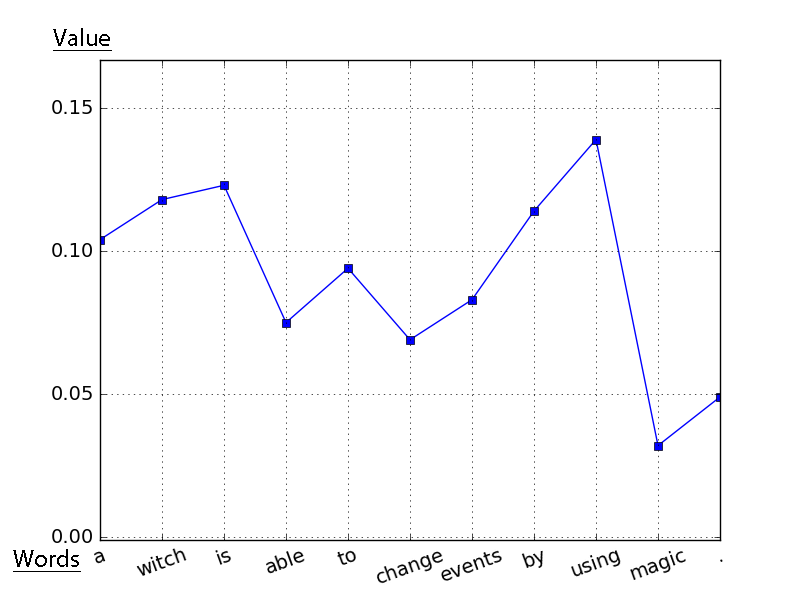
\includegraphics[width=.48\textwidth]{chapter4_experiments/images/sem-val1.png}
}
\subfigure[book - catalogues]{
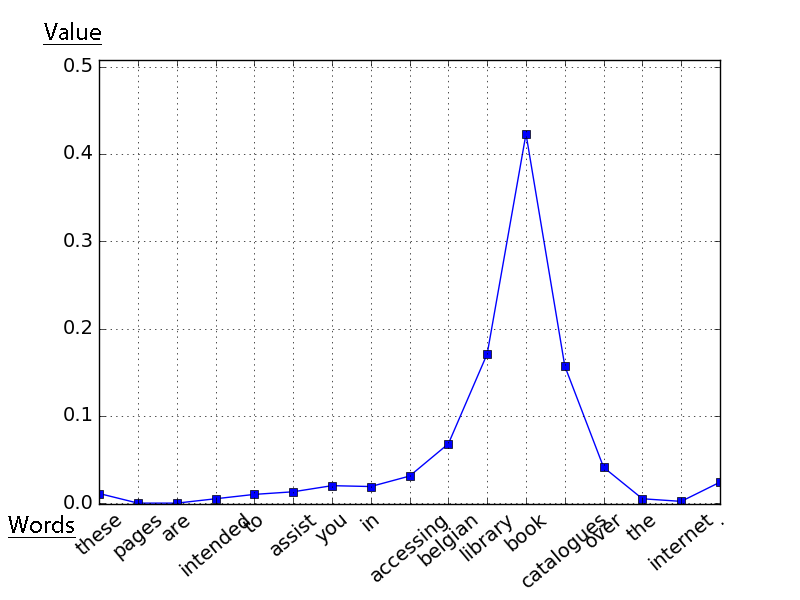
\includegraphics[width=.48\textwidth]{chapter4_experiments/images/sem-val2.png}
}
\subfigure[plant - storage unit]{
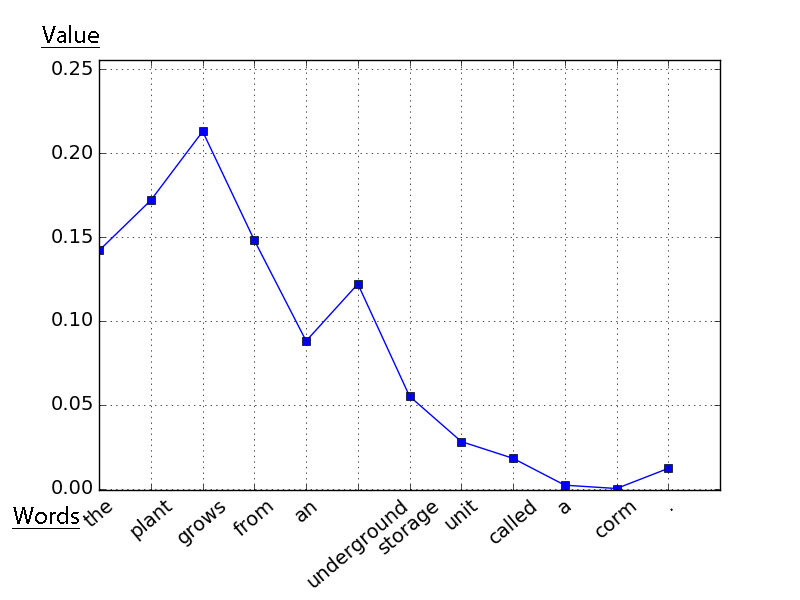
\includegraphics[width=.48\textwidth]{chapter4_experiments/images/sem-val3.png}
}
\caption[Semantic values, general domain supervised experiments]{Corresponding plots for three selected sentences from the test set of SemEval2010 for calculation of semantic values for words in the sentence.}
\label{fig:semantic-val}
\end{figure}

\paragraph{Scores distribution} This experiment is described in Subsection \ref{subs:score-distr}. It helps to look into the differences of scores given by the network to the relational classes.
The Figure \ref{fig:scores-distr} shows it for the same three examples, that were used for the 
experiment with semantic values. The first sentence is correctly classified and it can be seen, that all other scores are 
negative and only the correct class gives a comparatively large positive score. The second sentence 
distribution shows that network was hesitating between two acceptable classes and thus it 
got two small, but positive scores for both of them. The third sentence was recognised as 
''Other'',
 thus all the scores have to be negative. But two classes got very small negative scores, that are 
 correct class ''Entity-Origin'' and very close to the context of the sentence ''Product-Producer''.

\begin{figure}[H]
\centering
\subfigure[InstrumentAgency]{
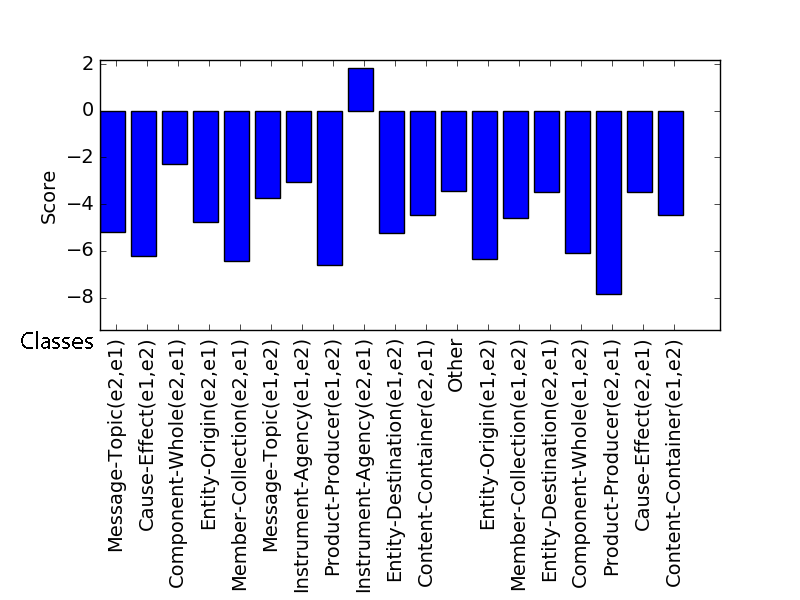
\includegraphics[width=.47\textwidth]{chapter4_experiments/images/scores1.png}
}
\subfigure[ComponentWhole]{
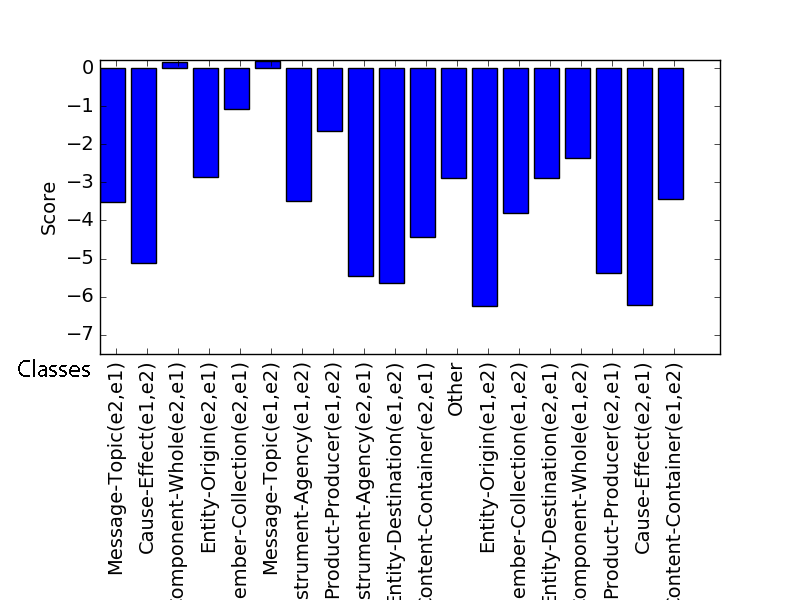
\includegraphics[width=.47\textwidth]{chapter4_experiments/images/scores2.png}
}
\subfigure[EntityOrigin]{
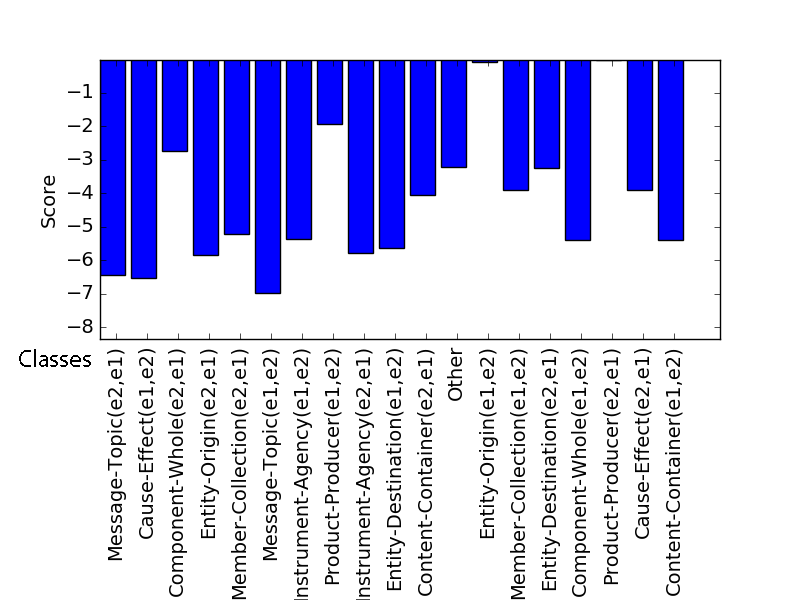
\includegraphics[width=.47\textwidth]{chapter4_experiments/images/scores3.png}
}
\caption[Scores distributions, general domain supervised experiments]{Scores distributions of relational classes for three chosen sentences from the test set of SemEval2010.}
\label{fig:scores-distr}
\end{figure}



\section{Supervised training evaluation, medical domain}
These experiments were held to check the applicability of the ranking CNN to the medical 
domain. Thus several popular medical datasets for Relation Extraction were chosen and 
evaluation compared to existing results.
There are a lot of relational classes specific only for medical domain. One of the most popular ones 
is about a general interaction between different entities, such as proteins, genes, drugs. Each 
interaction can have numerous more specific subclass relations, but for now tests are performed 
on generic relations. One more considered dataset contains \textit{treatment-for} and 
\textit{prevents-from} relations, that are very interesting by having high granularity level, i.e. 
they are very close by meaning.
\subsection{AIMed}
AIMed dataset was a result of research in \cite{bunescu2005comparative}.  The authors are 
concerned with automated information extraction from medical texts, especially information about 
human genes/proteins. They chose to think of genes and proteins as interchangeable ideas 
because there is a direct correspondence between them. To obtain the dataset, the authors manually 
tagged about one thousand Medline abstracts \footnote{\url{https://www.nlm.nih.gov/bsd/pmresources.html}}.
They mention following sources of abstracts for human protein interactions:
\begin{enumerate}
  \item 200 abstracts that are known to contain protein interaction from the Database of Interacting Proteins
  \item 30 abstracts for negative examples, where more than one protein mentioned, but there is no interaction between them
\end{enumerate}
In such a way, the AIMed dataset consists of abstracts with marked proteins and protein 
interactions as  pairs. For example

  \begin{verbatim}
    In contrast , in the absence of <prot>  p21ras </prot>  
    , coexpression of <prot>  JAK2 </prot>  and <prot>  
    Raf - 1 </prot>  resulted in an overall decrease in 
    the <prot>  Raf - 1 </prot>  kinase activity .
  \end{verbatim}

has several marked proteins, but no relations. And this

\begin{verbatim}
    Under these conditions , a ternary complex of 
    <p1  pair=6 >  <prot>  p21ras </prot>  </p1>  , 
    <p2  pair=6 >  <prot>  JAK2 </prot>  </p2>  , 
    and  <prot>  Raf - 1 </prot>  was observed .
  \end{verbatim}
  
has three proteins and one interaction pair in it. Since the experiments require sentences with 
only two marked entities the dataset was preprocessed before usage. Each marked entity in the 
sentence was considered as the first entity with each other entity as the second one. Each 
pair was considered only once in the order they are mentioned. An example was marked positive if
proteins were in the same ''pair'' number as ''p1'' and ''p2'' nodes and negative otherwise. In 
the case of presence of ''p1'' or ''p2'' tags, only proteins in these tags were considered, as the 
number of negative samples is significantly larger anyway.  So 
from the first aforementioned sentence six negative examples would be obtained, with entity 
pairs ''p21ras'' - ''JAK2'', ''p21ras'' - ''Raf - 1'' (first occurrence), ''p21ras'' - ''Raf - 1'' (second occurrence), ''JAK2'' - ''Raf - 1'' (first occurrence), ''JAK2'' - ''Raf - 1'' (second occurrence), 
''Raf - 1'' (first occurrence) - ''Raf - 1'' (second occurrence). In the case of the second sentence,
one positive example would be generated with entity pair ''p21ras'' - ''JAK2''.

The dataset is highly unbalanced, having much more negative examples, than positive ones. 
But as all the evaluation tests in other papers are done without balancing, so were held the 
experiments in here.

\subsection{DDI}
The second important relation in medical domain is a drug interaction. The drug interaction is observed 
when one drug influences the level of activity of the other drug \cite{segura20111st}. Knowledge 
about drug 
reactions is critical for patient safety and healthcare costs. There are drug databases, for example, 
DrugBank database \footnote{\url{https://www.drugbank.ca/}}, but data in them is not always up 
to date. 
New information is published regularly in reports and articles. The authors of \cite{segura20111st} are concerned with the application of automatic Natural Language Processing tools for 
extracting knowledge about drug interactions from textual data. Therefore gold standard 
dataset for training machine learning models was created. This dataset 
consists of manually annotated with interactions DrugBank database texts, where drugs were marked by MetaMap 
tool \footnote{\url{https://metamap.nlm.nih.gov/}}. The example of an annotated sentence is:

\begin{verbatim}
<sentence id="DrugDDI.d27.s0" origId="s0" text="The concomitant 
  intake of alcohol and Acamprosate does not affect the 
  pharmacokinetics of either alcohol or acamprosate.">
<entity id="DrugDDI.d27.s0.e0" origId="s0.p1" charOffset="26-33"
 type="drug" text="alcohol"/>
...
<pair id="DrugDDI.d27.s0.p0" e1="DrugDDI.d27.s0.e0" 
e2="DrugDDI.d27.s0.e1" interaction="false"/>
...
</sentence>
\end{verbatim} 

So for each sentence drugs are marked and then all possible pairs with indication of interaction 
between entities - either ''true'' or ''false''. For the test dataset, interaction is set to ''?'' and in separate 
file with gold annotations the labels are written down.

In order to use the dataset each sentence was repeated as many times as it has pairs and for 
each case only one pair of entities was marked. Labels were given according to the 
corresponding interaction label. Again, as with AIMed, the dataset is very unbalanced, having 
more negative examples than positive. But as evaluation papers use exact unbalanced test set 
balancing was not performed.

\subsection{Rosario-Hearst dataset}
This medical dataset was developed for the research in \cite{rosario2004classifying}. Initially, 
the dataset was obtained from MEDLINE abstracts and manually labeled by an expert for seven 
possible relations between DISEASE and TREATMENT. Some of the sentences among the 
examples were also labeled as ''only disease'' or ''only treatment'' and some identified relations, 
such as ''no cure'' had too few examples. Thus the dataset was adapted for making experiments 
with Ranking CNN. First, all not binary relations were filtered out. Then among them only large 
enough were left, they are ''treatment for'' and ''prevents from''. All the other binary relations were 
united for the class ''Other''. Finally, the dataset includes 810 sentences labeled as ''treatment for'', 
63 sentences labeled as ''prevents from'' and 69 for ''Other''. Dataset also contained ''not relevant'' 
examples, i.e. sentences that simply do not contain any entities or relations at all. These examples were outnumbering any of classes, but they could not be used for the experiments with the Ranking Convolutional Neural Network.

This dataset was initially represented as a set of sentences with two (or less) marked entities for each sentence, so the transformation for the experiments was straightforward.

\subsection{Results}
\label{subs:med-superv-res}
 Validation tests were held on AIMed dataset at the same setup as for general domain. But also 
one more choice was tested - usage of general domain embeddings and embeddings trained on 
PubMed abstracts dump from December 2016. The resulting F1 scores could be seen in the 
Table \ref{tab:val-aimed}.

\begin{table}
        \centering
        \begin{tabular}{|c|c|c|c|c|c|c|}
          \hline
            & \multicolumn{6}{|c|}{General domain embeddings} \\\hline
            & \multicolumn{3}{|c|}{Word embedding size 300} & \multicolumn{3}{|c|}{Word embedding size 400} \\\hline
            Dist. emb. & GloVe & Word2Vec & Swivel & GloVe & Word2Vec & Swivel  \\\hline
            \multicolumn{1}{|c|}{30} & 92.295 & 90.04 & 92.12 & 91.86 & 86.72 & 92.76 \\\hline
            \multicolumn{1}{|c|}{40} & 92.49 & 89.74 & 92.05 & 92.09 & 85.49 & 93.00 \\\hline
            \multicolumn{1}{|c|}{50} & 92.36 & 89.19 & 91.87 & 92.09 & 85.13 & 91.27 \\\hline
            \multicolumn{1}{|c|}{70} & 92.62 & 87.65 & 92.07 & 91.797 & 87.099 & 91.32 \\\hline
        \end{tabular}
        
        \begin{tabular}{|c|c|c|c|c|c|c|}
          \hline
            & \multicolumn{6}{|c|}{Medical domain embeddings} \\\hline
            & \multicolumn{3}{|c|}{Word embedding size 300} & \multicolumn{3}{|c|}{Word embedding size 400} \\\hline
            Dist. emb. & GloVe & Word2Vec & Swivel & GloVe & Word2Vec & Swivel  \\\hline
            \multicolumn{1}{|c|}{30} & 91.97 & 91.71 & 92.43 & 91.65 & 91.56 & \textit{93.25} \\\hline
            \multicolumn{1}{|c|}{40} & 92.44 & \textit{92.13} & \textit{92.72} & \textbf{93.38} & 91.23 & 92.46 \\\hline
            \multicolumn{1}{|c|}{50} & 92.19 & 91.397 & 92.51 & 91.85 & 91.92 & 92.55 \\\hline
            \multicolumn{1}{|c|}{70} & \textit{92.84} & 90.95 & 92.47 & 92.19 & \textit{92.197} & 91.7 \\\hline
        \end{tabular}
        \caption[Cross-validation for the medical domain]{Results of the cross-validation experiments on AIMed dataset obtained by simple calculation of F1-score for binary case. Every score is an averaged score of four 
experiments. First table contains results for general domain embeddings, second for medical 
domain. With \textit{italics} marked scores maximal in the column and \textbf{bold} is for the 
maximal result overall.}
        \label{tab:val-aimed}
    \end{table}

All the training accuracies reached 100 percent, sometimes after 4-5 epochs, except for experiments with Word2Vec of length 400 trained on general domain. In those experiments accuracy was reaching 94-96 percents.
From the results of the evaluation, it can be seen that embeddings trained on medical domain always 
give better result. The highest results are also always obtained with GloVe embeddings, while changing 
the dimensionality of word embeddings does not critically change the score. Change in the size 
of distance embeddings causes worse results when getting higher than 50. As the best model 
was chosen the one with GloVe medical embeddings of size 400 and with distance embeddings 
of 40.

As in the original paper \cite{bunescu2005comparative} results were obtained by 10-fold 
cross-validation and models in several other papers were as well 
(\cite{bunescu2005subsequence}, \cite{airola2008all}) evaluated in this way, the test for AIMed 
dataset was also performed with original 10-fold split. The DDI dataset also contains direct split on 
training and testing articles, so all the sentences formed from the testing articles were used as a 
testing set. The Rosario-Hearst dataset was simply split to 75\% of training data and 25\% of testing 
data and evaluation was held on the testing data. The results of testing 
the network are in the Tables \ref{tab:test-aimed}, \ref{tab:test-ddi}, \ref{tab:test-ros-hearst}.

\begin{table}[h]
  \begin{center}
 \begin{tabular}{ | c | c | c | c | }
    \hline
    Classifier & P & R & F1 \\ \hline
    Original paper best result \cite{bunescu2005comparative} \footnote{As in both \cite{bunescu2005comparative} and \cite{bunescu2005subsequence} authors gave PR-curve for result evaluation here was used the point corresponding to P=55.69 as obtained by the Ranking CNN.} & 55.69 & 36 & 43.73 \\\hline
    Subsequent kernels \cite{bunescu2005subsequence} & 55.69 & 54 & 54.83 \\\hline
    Graph kernel \cite{airola2008all} & 52.9 & 61.8 & 56.4  \\ \hline
    Supervised Ranking CNN (balanced train) \footnote{Training was performed on the dataset where number of negative and positive examples was balanced by cutting off negative examples.} & 34.27 & \textbf{90.56} & 49.29 \\ \hline
    Supervised Ranking CNN  & 55.69 & 63.85 & \textbf{58.38}  \\ \hline
    \end{tabular}
    \caption[Medical domain, AIMed evaluation results]{Results of evaluation of the network with AIMed.}
\label{tab:test-aimed}
\end{center}
\end{table}

\begin{table}
  \centering
     \begin{tabular}{ | c | c | c | c | }
    \hline
    Team \footnote{Results of competition from the original paper \cite{segura20111st}} & P & R & F1 \\ \hline
    WBI &  60.54 & 71.92 & 65.74 \\ \hline
    FBK-HLT &  58.39 & 70.07 & 63.70 \\ \hline
    Uturku &  58.04 & 68.87 & 62.99 \\ \hline
    LIMSI-CNRS &  55.18 & 64.90 & 59.65 \\ \hline
    laberinto-uhu &  50.00 & 44.37 & 47.02 \\ \hline
    Supervised Ranking CNN (balanced train) & 22.38 & \textbf{100.00} & 36.58 \\ \hline
    Supervised Ranking CNN & \textbf{91.75} & 98.68 & \textbf{95.09} \\ \hline
    \end{tabular}
  \caption[Medical domain, DDI evaluation results]{Results of evaluation of the network with DDI.}
\label{tab:test-ddi}
\end{table}

\begin{table}
  \begin{center}
      \begin{tabular}{ | c | c | c | c | }
    \hline
    Classifier & P & R & F1 \\ \hline
    Supervised Ranking CNN & 90.05 & 82.14 & 85.58 \\ \hline
    \end{tabular}
\caption[Medical domain, Rosario-Hearst evaluation results]{Results of evaluation of the network with Rosario-Hearst dataset.}
\label{tab:test-ros-hearst}
\end{center}
\end{table}

For the training datasets, all the experiments were getting 100 percent accuracy. 

It is interesting to notice, that training on the balanced dataset while testing still on unbalanced 
leads to higher Recall, but lower Precision. It directly reflects the idea, that distribution of both 
training and testing sets should be the same, otherwise supervised learner will not be able to 
be precise. So having a balanced training set, model suggests that much more examples are 
positive in the testing set than it really is - from what follows high Recall. But this time it is not the 
case and that is why Precision is low.

Also, it should be noticed, that in the AIMed and DDI datasets one and the same sentence will be an 
example for both negative and positive labels. And of course, it is hard for the network to extract 
syntactic construction that will be a sign of positive relation. 

So it can be concluded, that the model gives state-of-the-art results for various medical 
datasets with different classes of relations. Compared to the evaluation from several other authors Ranking
CNN gives always a better result. 


\subsection{Interpretation}
\paragraph{Representative trigrams extraction} 
In order to see the effect of balancing datasets, several sets of representative trigrams were 
extracted. 

The first one is for the network trained on the balanced AIMed dataset, second one is for the unbalanced 
dataset and the third one was made as a separate experiment, where dataset was initially 
balanced and then split on 75\% for training and 25\% for testing. The result shown by this 
training was P=51.91, R=92.08, F1=66.39.

\textbf{Balanced dataset} \textit{interaction with p25shc, binding, complex, interaction}

\textbf{Unbalanced dataset} \textit{interaction of the, interaction with p25shc, binding, binding region of}

\textbf{Initially balanced dataset} \textit{tr6 specifically binds, interacts poorly with, interacts with the, interaction}

From the human point of view, all the sets capture a lot of meaningful expressions of interaction.

The same three sets were obtained for DDI dataset. The scores for the network trained on 
the initially balanced dataset are P=59.68, R=98.84, F1=74.42, so it performs better than on 
AIMed dataset. But of course, it should be noticed that in general results for DDI dataset are also 
higher.

\textbf{Balanced dataset} \textit{of aprepitant with, hormonal contraceptives may, of erythromycin and, taking tarceva with, of erythromycin with, probenecid is, amphetamines may, azithromycin had, the benzodiazepines may}

\textbf{Unbalanced dataset} \textit{etonogestrel may interact, monoamine oxidase inhibitors, barbiturates, of erythromycin with, of amphetamines, nsaids can reduce, carbamazepine, may inhibit, nsaids may diminish}

\textbf{Initially balanced dataset} \textit{caution, agents, drugs, inhibitors, amphetamines, levels}

For DDI dataset most meaningful are trigrams extracted for the unbalanced training set. It can be explained by considering the fact, that the unbalance in amounts of negative and positive examples for this dataset are higher (almost 15 times more negative examples), than for the AIMed (around 3 times more negative examples). So when balancing is performed, network learns more drug names that can affect each other, rather than syntactic constructions denoting interactions.

\paragraph{Semantic values} 
For checking how the network ''sees'' the sentence in terms of values for the final decision 
two examples from AIMed test dataset were taken. The first one was classified correctly and the 
second one was mistakenly classified as ''Interaction''. The sentences are:

\begin{itemize}
  \item "Our data suggest that TR6 inhibits the interactions of $<e1>$LIGHT$</e1>$ with $<e2>$HVEM$</e2>$ / TR2 and LTbetaR, thereby suppressing LIGHT - mediated HT29 cell death."
  \item "We have previously identified $<e1>$IL - 11$</e1>$ specific binding protein which is distinct from that of $<e2>$IL - 6$</e2>$ in a number of cell lines."
\end{itemize}

Corresponding plots for these examples can be seen in the Figure \ref{fig:aimed-semantic-val}. The 
first sentence classified correctly as denoting ''Interaction'' and it can be seen that there are  
spikes over \textit{inhibits} and \textit{interactions of} and \textit{with}. As the value calculated for the trigram, it would be visualised over the central word of it. Thus, spike in the centre over \textit{/} is a spike over a protein name \textit{hvem/tr2}. That denotes that network is learning entities names as well. The second example is classified wrongly as describing interaction. 
The plot has numerous spikes over names of proteins and over \textit{specific binding protein} that leads to the high score for the 
''Interaction'' class, while these exact proteins do not interact.

Additionally, it is seen, that with longer sentences semantic values become much smaller (compare to 
analogous evaluation for SemEval2010 dataset in general domain) because they are distributed 
among all the words and thus it is harder to extract needed parts. Due to this spikes over the beginning and the end of 
an example become more prominent. They appear because sentences are padded with zero values for convolution and the 
activation function is tanh. Thus, zeroes can get higher values than some other words in the sentence with negative 
values.

\begin{figure}[H]
  \tiny
\centering
\subfigure[LIGHT - HVEM]{
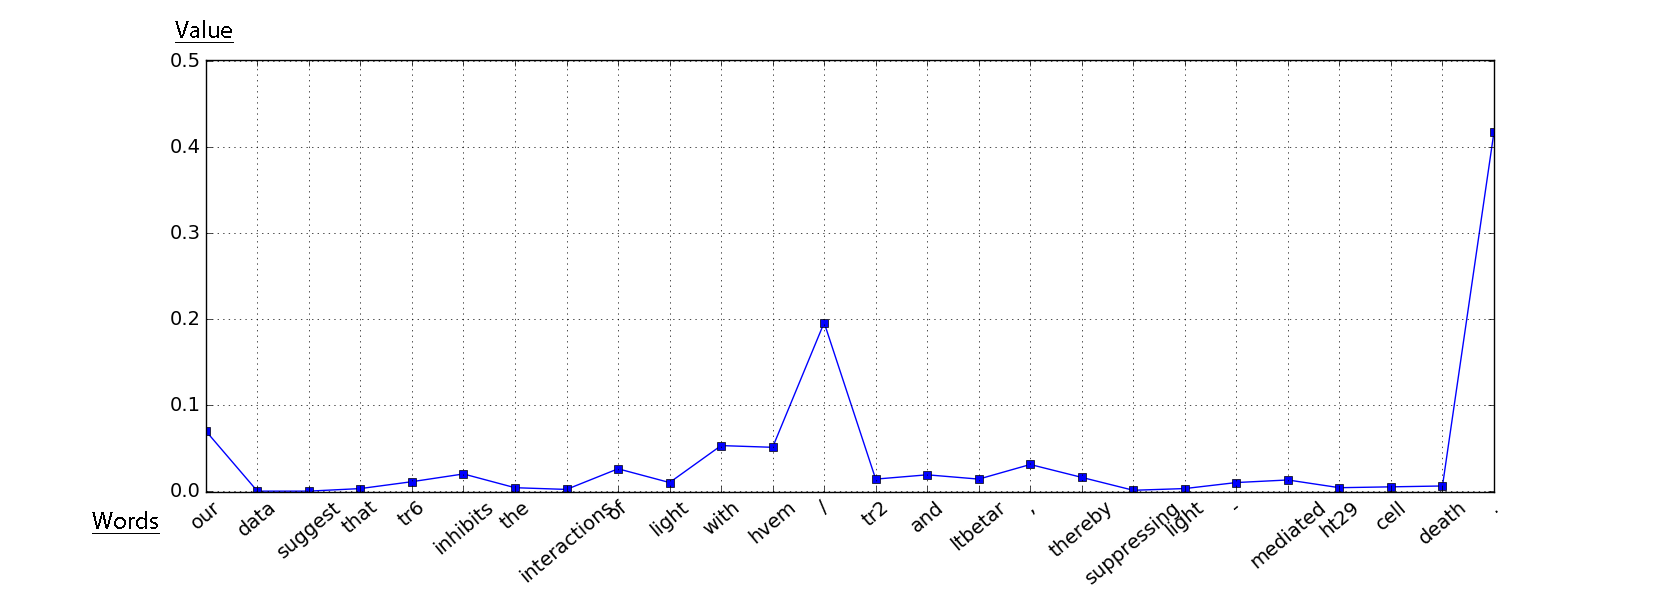
\includegraphics[width=\textwidth]{chapter4_experiments/images/aimed-sem-val1.png}
}
\subfigure[IL-11  - IL-6]{
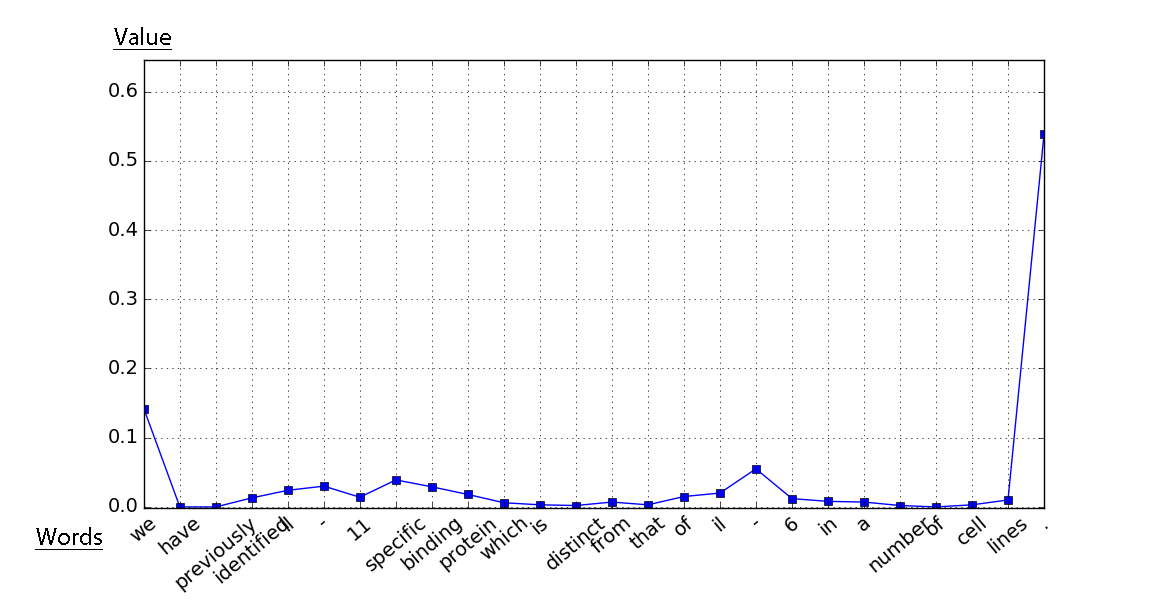
\includegraphics[width=0.75\textwidth]{chapter4_experiments/images/aimed-sem-val2.png}
}
\caption[Semantic values, medical domain supervised experiments]{ Semantic values for classification of the words in sentences. }
\label{fig:aimed-semantic-val}
\end{figure}

\paragraph{Scores distribution}
Corresponding scores distribution plots for the same two examples can be seen in the Figure 
\ref{fig:aimed-scores-distr}. The first example was recognised correctly and the network is quite 
sure in its answer. The second one was recognised 
incorrectly with a rather high certainty as well. This again can be explained by the spikes on the protein names 
that are seen on the semantic evaluation plot for the second example.

\begin{figure}[H]
\centering
\subfigure[Interaction]{
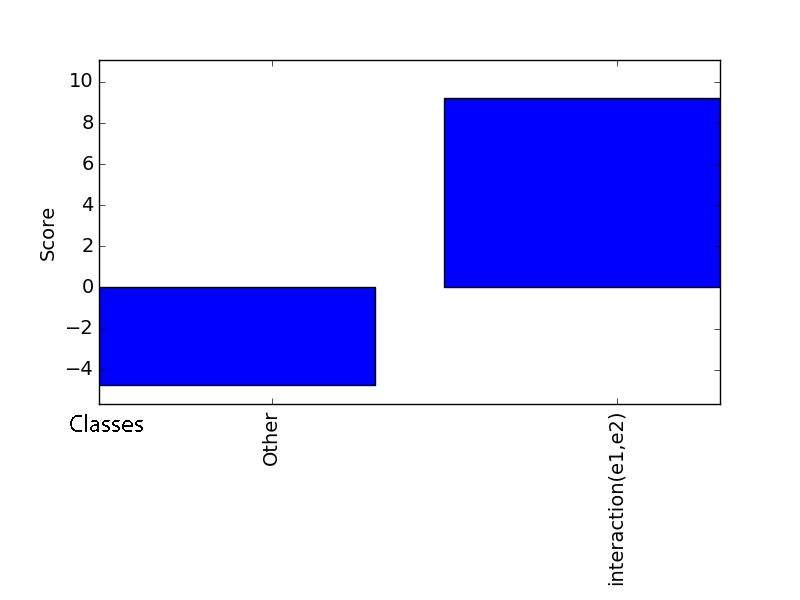
\includegraphics[width=.47\textwidth]{chapter4_experiments/images/aimed-scores1.png}
}
\subfigure[Other]{
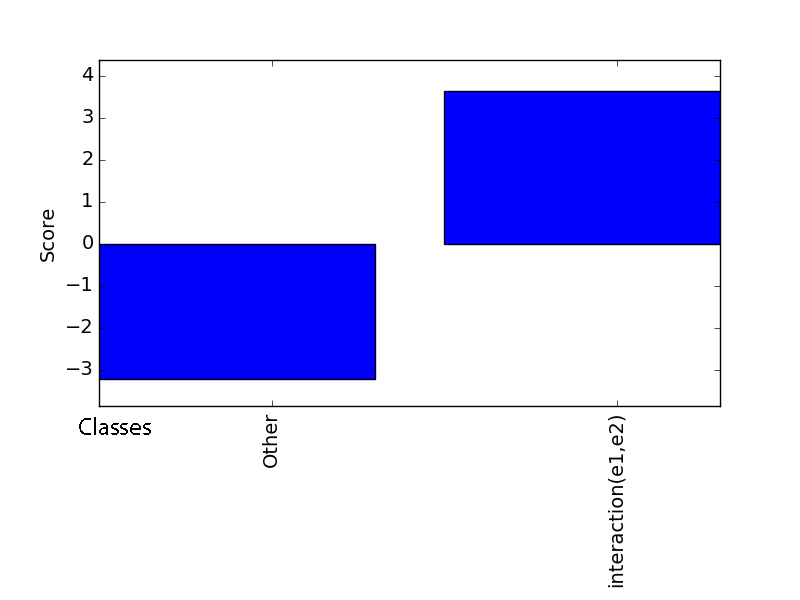
\includegraphics[width=.47\textwidth]{chapter4_experiments/images/aimed-scores2.png}
}
\caption[Scores distributions, medical domain supervised experiments]{Distribution of scores values.}
\label{fig:aimed-scores-distr}
\end{figure}


\section{Distant supervision evaluation}
The question to answer by these experiments is the possible quality of the model trained 
distantly. Also, possible ways of creating distantly supervised data are described.
\subsection{General domain: KBP37 based distantly supervised dataset} 
As it was mentioned before KBP37 dataset was adapted from the MIML-RE dataset from 
\cite{angeli2014combining}. In order to evaluate Distant Supervision in general domain, this dataset was 
chosen, as authors of \cite{angeli2014combining} made publicly available the set of relation 
pairs that were used for the creation of the dataset. They used 2010 and 2013 TAC KBP \footnote{\url{https://www.ldc.upenn.edu/collaborations/current-projects/tac-kbp}} documents as a source of relations. 
For creating the supervised dataset they utilised Amazon Mechanical Turk \footnote{\url{https://www.mturk.com/mturk/welcome}} for labelling examples that they got after aligning entity pairs to 
sentences from 2013 Wikipedia dump. They annotated 23725 examples, that were transformed to 
KBP37 dataset by \cite{DBLP:journals/corr/ZhangW15a}.

A closer investigation of the entity pairs from TAC KBP showed that the quality of them is 
not high enough. For example, they could contain only one letter as a name or just a word ''president'' as an entity 
for ''org:top-members/employees'' relation.
Thus as a Knowledge Base for Distant Supervision experiments both relational pairs from MIML-RE 
\footnote{\url{https://nlp.stanford.edu/software/mimlre.shtml}}, i.e. from TAC KBP, and Wikidata 
\footnote{https://query.wikidata.org/} were used. Wikidata returned fewer pairs 
corresponding to required relations, but they are more precise. Entity pairs from Wikidata were 
queried through the query interface for each of the corresponding relations.  
The amount of entity pairs for each of the relation types varies a lot - from less than 1000 to more than 
50000. For creating the ''Other'' class were chosen ''per:religion'', ''per:children'', ''org:political/religious-affiliation'' 
entity pairs. In order to minimise noise effect of not accurate entity pairs from TAC KBP, 
the entity pairs containing one letter entities or names consisting only of capital letters with dots were filtered out and not used.

For raw text corpus the NewYork 
Times archive \footnote{\url{https://catalog.ldc.upenn.edu/ldc2008t19}} was taken.
According to the idea of the 
Distant Supervision an alignment of entity pairs from a Knowledge Base to the text should be performed. This was done by the 
simple method of string matching. It means that entities' names were simply searched 
in the textual corpus. If sentence included two entities that are related according to the Knowledge Base that would give an example
for the corresponding relation.
In order to implement the lookup of the words in a large volume of textual data, Whoosh, a python library for 
indexing the text, was used \footnote{\url{https://whoosh.readthedocs.io/en/latest/}}. It allows to index 
each sentence of the text as a separate entry and then make a request to search for two 
entities' names and returns all the entries containing them. So, raw textual data 
from NYT corpora was split into sentences with NLTK library, indexed by 
Whoosh and then aligned with the set of entity pairs from the Knowledge Base. If all 
of the aligned sentences are taken, it would lead to a highly unbalanced, both by the amount of 
examples per relational class and the amount of examples per entity pair, and really huge dataset. That is why 
only 5 examples per entity pair were taken and the maximal amount of sentences in relational class 
was set to 3000. This resulted in a dataset with the overall amount of 75913 sentences. And even this dataset is 
already almost tree times more than the supervised dataset for the same relational classes and it was obtained 
completely automatically. It proves the point, that the amount of distantly supervised training data can be 
made as large as needed without any additional effort.

Apart from simple training on the distantly supervised data, several experiments for quality 
improvement were held: 
\begin{itemize}
  \item Applying Multiple Instance Learning. As it was explained in Subsection \ref{subs:mil}, training 
  examples for this setup are bags containing at least one correctly labeled sentence. Thus sentences 
  were grouped based on the entity pair they contain and each of this bags was labeled as 
  a relation, that this entity pair has in the Knowledge Base.
  \item Mixing supervised data. It was mentioned in \cite{riedel2010modeling} that distantly 
  supervised data introduces noise, but it was decided to check how adding existing 
  supervised data into the distant dataset would affect the training results.
  \item Using transfer learning. Generally, it might be a good idea to train the model on 
  existing supervised data and then continue tuning it with more and more distantly supervised data to get better results.
\end{itemize}

\subsection{Results}
\label{subs:gen-dist-res}
The results of training the network in various ways with distantly supervised data can be seen
in the Table \ref{tab:dist-gen-res}. For comparison, the supervised training result was also included in the 
table.

\begin{table}
  \begin{center}
 \begin{tabular}{ | c | c | c | c | }
    \hline
    Experiment & P & R & F1 \\ \hline
    Supervised training & \textbf{67.74} & 57.88 & \textbf{61.26} \\ \hline
    Distantly supervised training & 50.71 & 45.24 & 43.81 \\ \hline
    Distantly supervised + MIL & 51.82 & 46.61 & 45.40 \\ \hline
    Distantly supervised + supervised data & 57.64 & 57.84 & 55.03 \\ \hline
    Distantly supervised + supervised data + MIL & 60.25 & \textbf{58.24} & 56.93 \\ \hline
    Transfer from supervised & 48.93 & 44.14 & 42.73 \\ \hline
    Transfer from supervised + MIL & 51.13 & 44.92 & 44.58 \\ \hline
    \end{tabular}
\caption[General domain, Distant Supervision experiments results]{Precision, Recall and F1-scores for distantly supervised training evaluation.}
\label{tab:dist-gen-res}
\end{center}
\end{table}

The first conclusion that can be made - training without manually labeled data can be performed and 
it will achieve definitely higher results than random assignment (with the amount of classes 37 
F1-score for random assignment would be around 0.2\%). Thus it was successfully proven, that 
having publicly available Knowledge Base with required relation types and a large amount of textual data 
training set for a neural network solving the task of Relation Extraction can be constructed automatically. In
the context of the task to continuously extract new knowledge from newly published texts, this approach is 
more appealing than manual extraction. Supervised training might give better results but it still 
requires the manually curated creation of training dataset, that is most of the times not possible and also 
should be repeated for any new relational class. Also, in real-world application, while validating the 
results for including into a Knowledge Base not only the top score answer might be considered. Thus, 
if only top one considered as an answer ratio of correct answers is 42.99\%. If top three answers 
are considered for checking, then already 68.14\% will be recognised correctly. Further addition does 
not change the result so much - with top five the percentage of correct answers is 79.58\%.

The second point is a definite positive effect of Multiple Instance Learning. Every time when Multiple Instance Learning was applied the previous result 
was improving by approximately two percents. Good point also that not only Precision or 
Recall alone is improved, but both simultaneously. It can be concluded, that exploration of further more complex 
methods for noise reduction in the distantly supervised data will significantly improve the score. 

The results of transfer learning experiment were disappointing, it performs even worse than 
simple distantly supervised training. It might be explained by different directions that datasets
are trying to lead the network - scopes of syntactic constructions in supervised dataset and in 
distantly supervised dataset might differ a lot. Thus pre-training with supervised data leads to a worse starting point for 
distantly supervised training than a random one.

As it was expected, mixing in existing supervised data improved drastically distantly 
supervised training. And also as expected, it gives a worse result than pure supervised training. But it should be 
pointed out that with Multiple Instance Learning together with mixed dataset setup, it was possible to reach higher Recall than for supervised 
training. This means that distantly supervised data helps the model to become more general, be 
less biased by the provided supervised dataset. It again might be a very good sign for live models, 
that are supposed to retrieve more and more new knowledge from new textual data, because
it is never possible to provide the needed amount of new labeled training data manually. 

\subsection{Interpretation}
\paragraph{Distantly and manually supervised datasets}
It is important, that manually supervised training and testing datasets are tightly coupled and they will have common 
context and common biases. Thus, evaluating distantly supervised model with existing testing
dataset might be not objective. There exist other ways to evaluate the results of Distant Supervision, for example, 
performed in \cite{Mintz:2009:DSR:1690219.1690287}, but they would not show a realistic comparison to the 
supervised results. Moreover, evaluation with supervised testing dataset allows having a fresh look at the 
quality of the supervised data. It might not be absolutely accurate, especially when the number of examples
is large. And the worst aspect is that the supervised training will cause bias to specific kind of mistakes (as they 
will be both in training and testing set).

Overall, if there exist a hypothetical full set of all possible syntactic constructions for describing a specific relation, 
supervised dataset would be some (most of the times not very big) subset of it and of course, 
it might contain errors of labelling, that both training and testing sets would share. On the 
other hand, distantly supervised dataset would be slightly different subset of the whole set, that 
might be spread more and more - thus evaluation with initial supervised testing set would be less 
and less objective, because some constructions that are not there would be recognised by the 
price of forgetting constructions from the supervised dataset. In general, this idea is reflected in the Figure \ref{fig:dist-superv-knowledge}.

\begin{figure}[H]
\centering
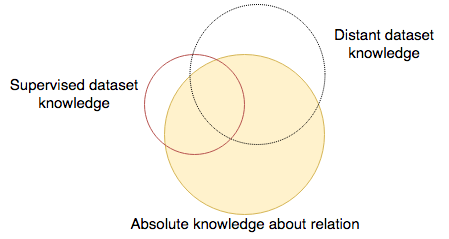
\includegraphics[width=250px]{chapter4_experiments/images/dist-superv-knowledge.png}
\caption[Relation of supervised and distantly supervised knowledge]{Concept of knowledge about a specific relation contained in supervised and distantly supervised datasets.}
\label{fig:dist-superv-knowledge}
\end{figure}

It seemed quite logical to suggest, that in order to have more basement for such conclusions one should look into the ratio of correctly
recognised examples for manually supervised and distantly supervised networks. The result of this investigation is depicted in the 
Figure \ref{fig:uniq-correct}. It can be seen, that for some of the relations manually supervised network will recognise much more 
constructions, but there are still relations for which distantly supervised network finds more constructions. Overall, a number of 
examples recognised only by the distantly supervised network is quite sensible. It can be concluded that the information contained 
in the distantly supervised dataset is useful and quite different from the one in the manually labeled dataset. Thus, the main 
goal when working with distantly supervised dataset is to get rid of the noise that lowers the precision of recognition.

\begin{figure}[H]
\centering
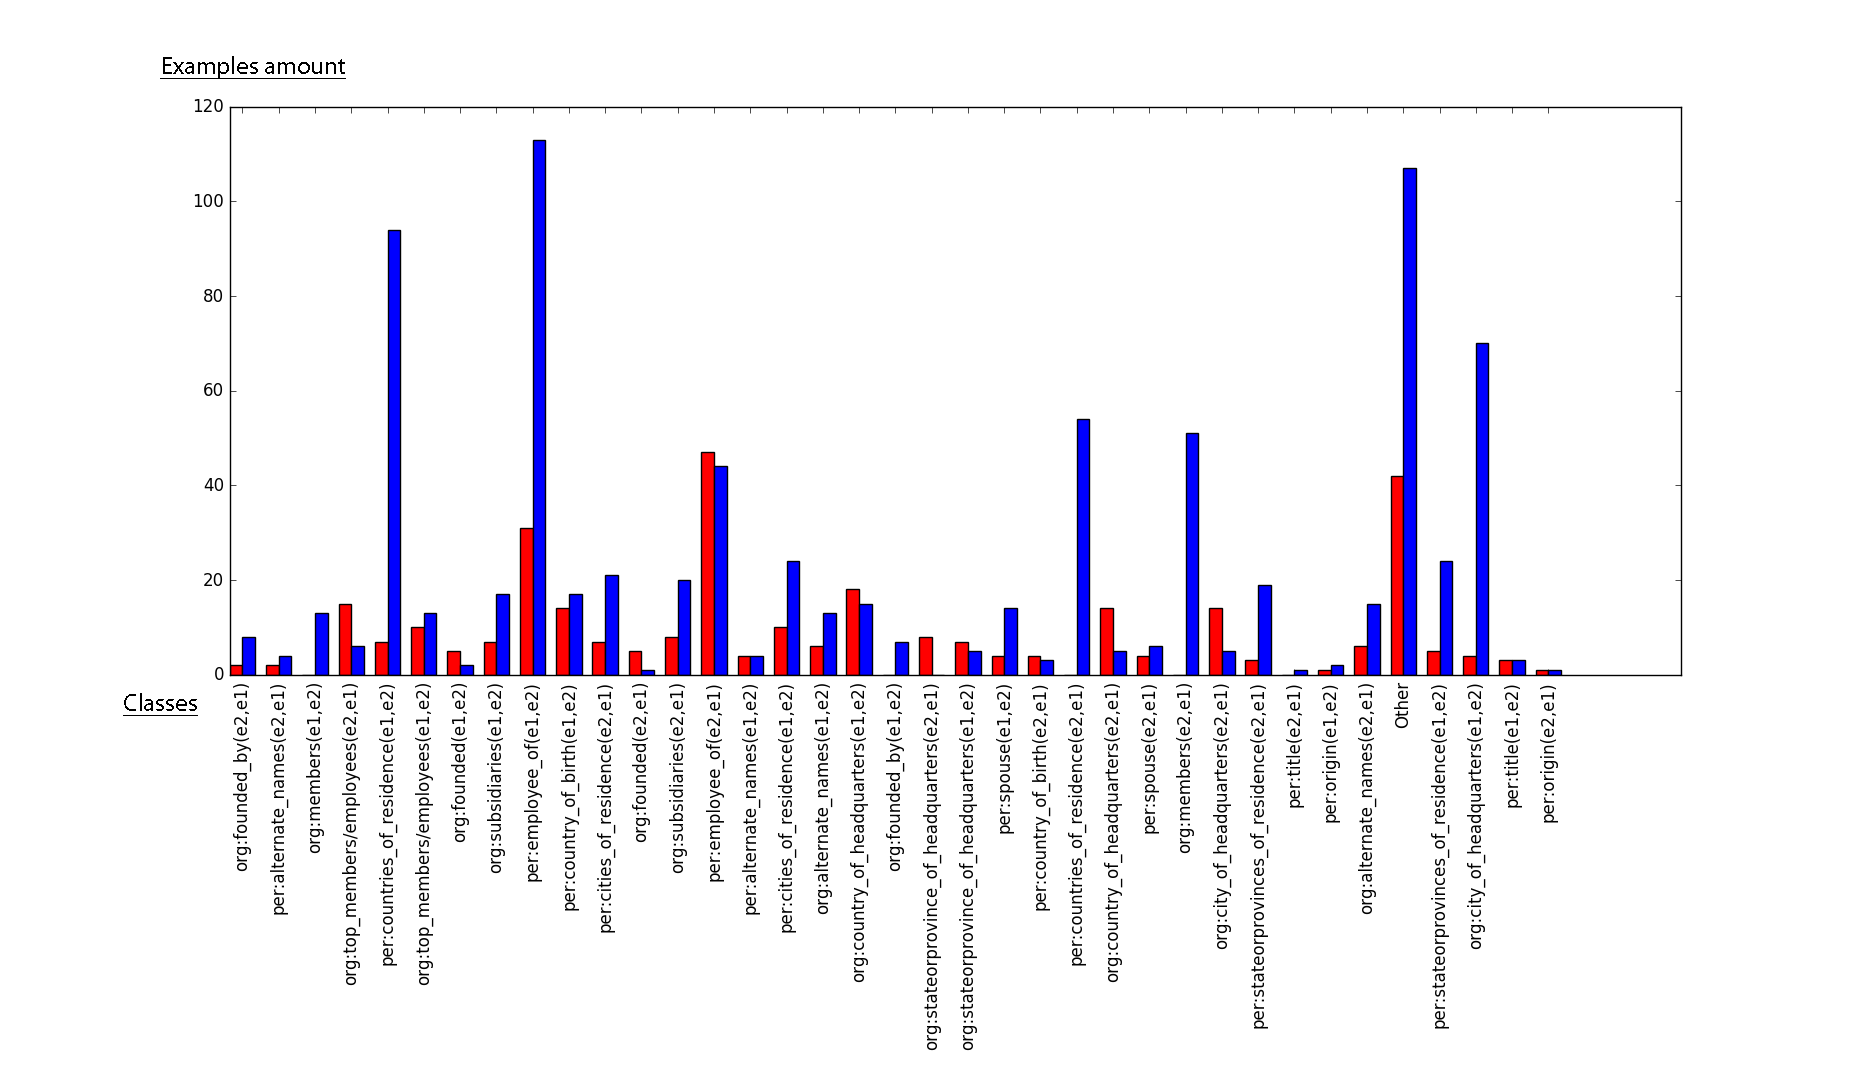
\includegraphics[width=\linewidth]{chapter4_experiments/images/uniq-correct.png}
\caption[Relation between correct answers for manually and distantly supervised training]{Blue bars show amount of testing examples that were recognised correctly by manually supervised network, but were not recognised by distantly supervised one. Red bars show the same amount for distantly supervised network.}
\label{fig:uniq-correct}
\end{figure}

\paragraph{Length of the examples}
\label{par:ex-length}
Of course one more very important aspect of relation recognition in a sentence is the length of the sentence and the distance
between the entities in it. The dependency can be seen in the Figure \ref{fig:dist-depend}. Spikes around the large values of length and  
distance are not representative, as the number of the examples there much smaller (3-5 sentences). But the overall the tendency 
is clearly seen - with the enlargement of the length or distance a number of errors grows and a number of right answers drops.
Any distantly supervised dataset will always be characterised by longer sentences on average, so this aspect should be taken into 
account when the dataset is constructed. For example, sentences longer than some limit can be simply not included in the 
final set of training examples.

\begin{figure}
\centering
\subfigure[Sentence length dependency]{
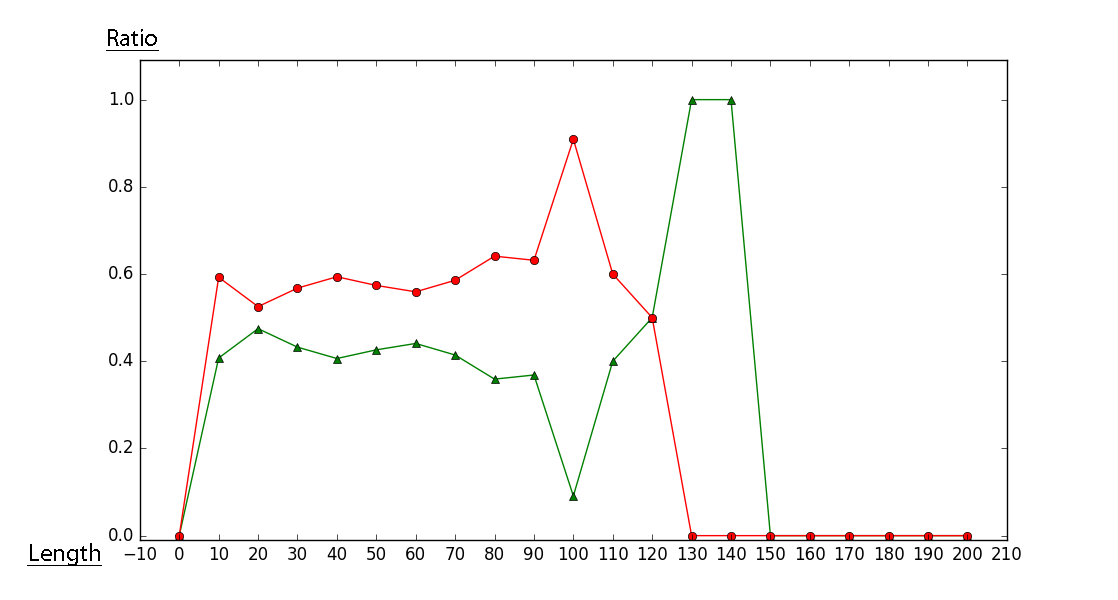
\includegraphics[width=.47\textwidth]{chapter4_experiments/images/length_errors.png}
}
\subfigure[Distance between entities dependency]{
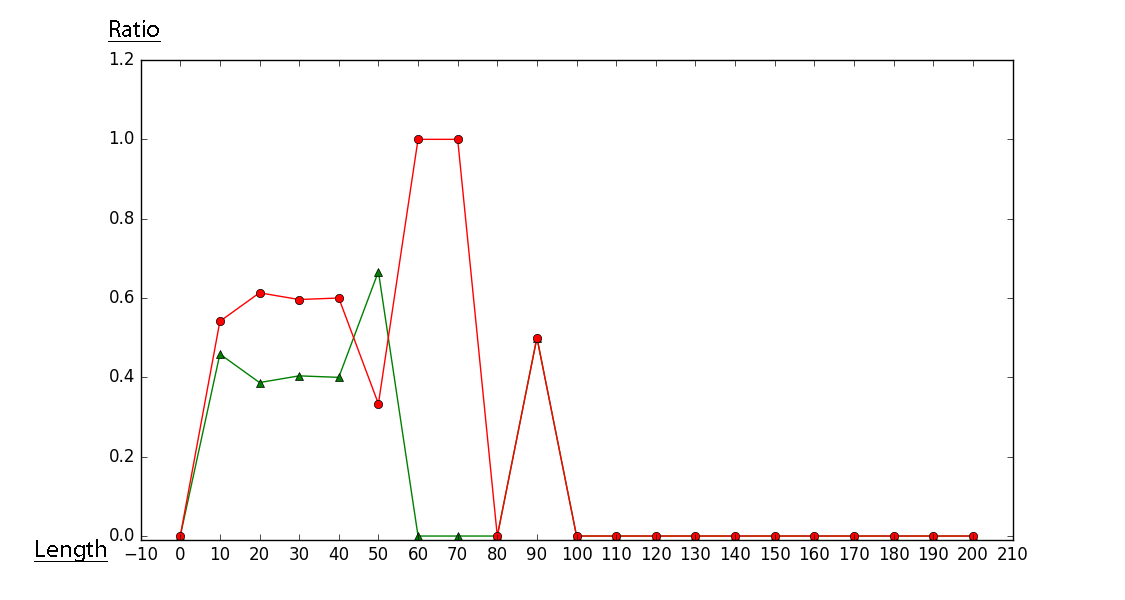
\includegraphics[width=.47\textwidth]{chapter4_experiments/images/betw_ent_errors.png}
}
\caption[Correlation of amount of correct and wrong answers with sentence length and distance between entities]{Dependency of the number of correct answers (green) and wrong answers (red) normalised by the overall amount of examples of specific length or with specific distance between entities correspondingly on the input sentence length and on the distance between entities.}
\label{fig:dist-depend}
\end{figure}

\paragraph{Representative trigrams}
If one takes a look at representative trigrams for the model trained on the distant dataset, mixed with 
supervised data and united in bags, several interesting observations can be made.
For example for relation ''per:spouse'', while supervised dataset obtained:

\textit{king george iii, his second wife, married gene raymond, wife melanie griffith, wife of actor, wife henrietta maria, husband jeff richmond, wife kimberly williams-paisley, wife of president}

newly trained model was able to obtain more general trigrams, such as:

\textit{wife of the, husband the, wife the, wife lee radziwill, wife of president, married yesterday to, wife of senator, wife of prime}

And the similar situation can be observed for several other relations. For example, 
''per:cities-of-residence'' becomes less unbiased in a sense of taking into account more cities, 
than it is in the training set.

\paragraph{Active learning}
\label{par:active-learn}
Even more interesting is an idea of exploiting representative trigrams as a tool for improving dataset. Thus, a look into 
representative trigrams obtained for the distantly supervised network can reveal some learned aspects that 
do not make sense from the human point of view. For example, for the relation ''org:founded-by'' found trigrams 
\textit{open society institute, fox broadcasting company, ethical treatment of, jack daniel's} seem to be 
not really representative. Same for the relation ''per:alternate-names'' a trigram \textit{mimi smith}. If these 
non representative trigrams are found in a sentence from the training dataset, the sentence might be 
filtered out, so the network will not learn the trigram anymore. A small experiment with two aforementioned 
relations showed improvement in scores. So, for ''org:founded-by'' Precision grew from 54.05 to 70 and 
Recall from 25 to 26.25. For ''per:alternate-names'' Precision improved from 33.33 to 38.24 and Recall 
from 21.74 to 28.26. This is a possibility to further improve Distant Supervision by application of Active Learning and iterative
transformations of the training dataset.
 


\subsection{Medical domain: Rosario-Hearst based distantly supervised dataset}
The Distant Supervision experiment setup for the medical domain was mainly performed according to 
\cite{roller2014applying}. Rosario-Hearst dataset was chosen as base supervised dataset 
because it contains more than two relations and relatively small that can allow evaluating the 
effect of adding distantly supervised data more. 

As a textual corpus, PubMed abstracts were used. The abstracts were downloaded without 
specialised search and only around 500000 were finally used for creating the dataset. 
In order to mark medical entities, MetaMap online tool 
\footnote{https://metamap.nlm.nih.gov/} was utilised. It allows to setup a lot of parameters for different 
output formats and text processing. As a simplest one, the Fielded MMI format was chosen. This 
format gives as an output all found entities, their unique identifiers in the MetaMap system Knowledge Base, 
their positioning in the text and additional information that was not used. It was chosen as it gives the least 
volume of the processed file and rather simple to use further. Also, it is important to notice that the input file was 
preprocessed with sentence tokeniser from NLTK toolkit, thus output was directly giving 
positions of the entities in each of the sentences.

The next step is to align a publicly available Knowledge Base to the preprocessed text. 
As entities marked with identifiers from MetaMap, relational base MRREL from the same source was used. This Knowledge Base 
\footnote{https://www.ncbi.nlm.nih.gov/books/NBK9684/} consists of many datasets 
and thus includes a lot of relational classes (almost 600). Among them ''may-be-treated-by'' and 
''may-be-prevented-by'' which correspond to ''treatment-for'' and ''prevents-from'' relations from 
the supervised dataset. So, entity pairs are taken from these two classes of MRREL Knowledge Base.
Then, with a Python script, all the tagged sentences that contain entity pairs with desired 
relations are separated. In order to construct examples for ''Other'' class, all possible pairs of entities
that are not in one of the classified relations according to the Knowledge Base were considered. Thus, a dataset containing 13025 
sentences was formed. For medical domain difference in sizes of the manually and distantly supervised
datasets is much larger, the distant dataset includes almost 16 times more examples than the manually
supervised one.

Using this distantly supervised dataset similar to the general domain experiments were 
performed with the supervised testing set for evaluation.

\subsection{Results}
The results of the training of the network in various ways with distantly supervised data can be seen
in the Table \ref{tab:dist-med-res}. For comparison, the supervised result also was included in the 
table.

\begin{table}[h]
  \begin{center}
 \begin{tabular}{ | c | c | c | c | }
    \hline
    Experiment & P & R & F1 \\ \hline
    Supervised training & \textbf{90.05} & 82.14 & \textbf{85.58} \\ \hline
    Distantly supervised training & 46.16 & 44.52 & 41.81 \\ \hline
    Distantly supervised + MIL & 59.67 & 50.24 & 54.17 \\ \hline
    Distantly supervised + supervised data & 76.81 & 67.62 & 70.45 \\ \hline
    Distantly supervised + supervised data + MIL & 87.68 & \textbf{83.33} & 85.3 \\ \hline
    Transfer from supervised & 54.07 & 48.57 & 51.17 \\ \hline
    Transfer from supervised + MIL & 61.84 & 43.33 & 49.29 \\ \hline
    \end{tabular}
\caption[Medical domain, Distant Supervision experiments results]{Precision, Recall and F1-scores for distantly supervised training evaluation.}
\label{tab:dist-med-res}
\end{center}
\end{table}

So it can be seen, that all the conclusions that were made for distantly supervised training in 
general domain, are also valid in the medical domain.

One interesting aspect of Rosario-Hearst dataset that it is highly unbalanced. The formed 
distantly supervised dataset is also unbalanced with the same relation ''treatment-for'' 
dominating over all others. It was interesting to see the effect of balancing of the dataset and the 
results of evaluation could be seen in the Table \ref{tab:dist-med-res-bal}.

\begin{table}[h]
  \begin{center}
 \begin{tabular}{ | c | c | c | c | }
    \hline
    Experiment & P & R & F1 \\ \hline
    Supervised training & \textbf{90.05} & 82.14 & 85.58 \\ \hline
    Distantly supervised training & 43.1 & 35 & 37.83 \\ \hline
    Distantly supervised + MIL & 56.22 & 60.24 & 55.87  \\ \hline
    Distantly supervised + supervised data & 85.35 & 86.43 & 85.88 \\ \hline
    Distantly supervised + supervised data + MIL & 84.17 & \textbf{89.05} & \textbf{86.45} \\ \hline
    Transfer from supervised & 46.95 & 45.95 & 40.76 \\ \hline
    Transfer from supervised + MIL & 60.14 & 43.57 & 50.53 \\ \hline
    \end{tabular}
\caption[Medical domain, Distant Supervision with balancing experiments results]{Precision, Recall and F1-scores for distantly supervised training evaluation with balanced distant dataset.}
\label{tab:dist-med-res-bal}
\end{center}
\end{table}

The results that were obtained by simply training on the balanced distant dataset are lower than for  
unbalanced one, but when the supervised data is mixed in the results become much higher. The first 
fact might be explained by the basic requirement of any supervised learner: the training and 
the testing dataset are supposed to be drawn from the same distribution. But the second fact can either mean that distantly 
supervised data is always uncertain, so true distribution of classes cannot be seen just from a number
 of examples, or that simple neglecting of some of the dominating class examples 
helped the network to avoid noisy data. Also, one point that was observed while constructing the distant dataset
is that the set of entity pairs for the relation ''treatment-for'' intersects with the set for ''prevents-from'' significantly.
Thus, there are a lot of examples in the dataset, that will be labelled with both of the relations, that confuses 
the network more when all the examples are included (in unbalanced setup). 

\paragraph{Representative trigrams} 
The representative trigrams also give the same intuition that was there in the general domain - 
distantly supervised data helps to avoid the biased understanding of the relations. So for the 
supervised training for relation ''prevents-from'' they were:

\textit{vaccine for pneumonia, vaccination against influenza, vaccination against swine, vaccine 
against pneumococcus, polio vaccination participation, influenza vaccination on, influenza 
vaccination, hepatitis b vaccine, vaccine 6}

They are clearly biased to various forms of vaccines and vaccinations. While for distantly 
supervised dataset mixed with supervised data were obtained:

\textit{malaria, nausea and vomiting, hiv-infected patients, tuberculosis, beclomethasone dipropionate, fluoride, cimetidine 1, ganciclovir}

These ones are not human-interpretable, but they are definitely not biased to 
vaccinations. The amount of disease and drug names in the trigrams reveals 
that it was not easy for the network to concentrate on the syntactic constructions for the 
relation itself rather than on the names of the entities. This can be explained by 
the bad choice of ''Other'' class examples. As all the sentences with various 
named entities were used for it, only sentences containing exactly diseases and 
drugs were classified for the relations and the network started to overfit on the 
entity names. One possible way to fight this problem is to replace entity names with 
certain keywords in all the examples. The experiment revealed, that this modification 
of the dataset lead to the improvement of the score for distantly supervised training. 
The score became P=52.06, R=52.38, F1=51.54 against 
P=46.16, R=44.52, F1=41.81 for non-modified dataset. Representative trigrams also 
show a very good progress:

\textbf{prevents-from}: \textit{entity1-resistant entity2, nausea and entity2, to prevent entity2, entity2, entity1 and entity2, use of entity2, entity1(entity2}

\textbf{treatment-for}: \textit{treatment of entity2, entity2, patients with entity2, treatment with entity1, treated with entity1, administration of entity1, response to entity1, entity2 with entity1}

But the result of the evaluation is lower than one for the non transformed dataset and with Multiple Instance Learning.
The problem with this approach is that Multiple Instance Learning cannot be applied anymore in the previous form, 
as all the entity pairs are the same and the examples cannot be grouped to form the bags on the 
basement of different entity pairs. But some other approaches might be explored, for example, 
randomly grouping some fixed amount of examples for one class into bags.


